

There are several benchmarks in the literature to be utilized for investigation of the numerical algorithms.
Benchmark solutions for impermeable rock have been constructed in \cite{Kemp,Linkov_4},
while that corresponding to the non-zero leak-off model with  $q_l$ vanishing at a crack tip has been
analyzed in \cite{MWL}.




In this paper, we introduce three different analytical benchmark
solutions cor\-res\-pond\-ing to the representations
\eqref{norm_leak_off_1}. Moreover, for each of the leak-off
functions under consideration we take two different
relationships between the injection flux rate $q_0$ and the leak-off
to formation $q_l$. In this way
 six different benchmark solutions are analyzed.

In order to formulate the benchmark solutions let us assume the
following form of the crack opening function:
\begin{equation}\label{w_bench}
w(t,x)=W_0(1+t)^\gamma h(x),\quad W_0=\sqrt[3]{\frac{3}{2}(3\gamma+1)},
\end{equation}
where $\gamma$ is an arbitrary parameter, and the function $h(x)$ ($0<x<1$) is given by:
\begin{equation}\label{w_0_bench}
h(x)=(1- x)^\frac{1}{3}+b_1(1-x)^{\lambda_1}+b_2(1-x)^{\lambda_2}.
\end{equation}
The choice of the next powers $1/3<\lambda_1<\lambda_2$ will depend on the
leak-off variant from \eqref{carter}. On consecutive
substitutions of \eqref{w_bench}-\eqref{w_0_bench} into the
relations \eqref{norm_speed}, \eqref{norm_boundary},
\eqref{w_system} and \eqref{new_speed} one obtains the remaining
benchmark quantities:
\begin{equation}\label{v_bench}
L(t)=(1+t)^{\frac{3\gamma+1}{2}},\quad V(t,x)=-W_0^3(1+t)^{\frac{3\gamma-1}{2}}h^2(x)\frac{\partial h}{\partial x}.
\end{equation}
\begin{equation}\label{q_0_bench}
q_0(t)=-W_0^4(1+t)^{\frac{5\gamma-1}{2}}\left(h^3\frac{\partial h}{\partial x}\right)|_{x=0}.
\end{equation}
\begin{equation}
\label{q_l_bench}
q_l(t,x)=W_0(1+t)^{\gamma-1}\times
\end{equation}
\[
\Big(\frac{3}{2}(3\gamma+1)\Big[\frac{1}{3}x\frac{\partial
h}{\partial x} +3h^2\left(\frac{\partial h}{\partial x}\right)^2
+h^3\frac{\partial^2 h}{\partial x^2}\Big]-\gamma h\Big).
\]



It can be easily checked that for $\lambda_1=1/2$ and $\lambda_2=4/3$
the leak-off function incorporates a square root singular term of
type \eqref{norm_leak_off_1}$_1$. By setting $\lambda_1=5/6$ and
$\lambda_2=4/3$ we comply with representation
\eqref{norm_leak_off_1}$_2$. Although in both of these cases
$q_{1(2)}^*$ exhibits a singular behaviour at the crack tip, it does
not detract from the applicability of our benchmarks. Finally, when
using $\lambda_1=4/3$ and $\lambda_2=7/3$, the benchmark gives a
non-singular leak-off function in the form
\eqref{norm_leak_off_1}$_3$.




\begin{figure*}[t]
        \centering
        \begin{subfigure}{0.32\textwidth}
                \centering
                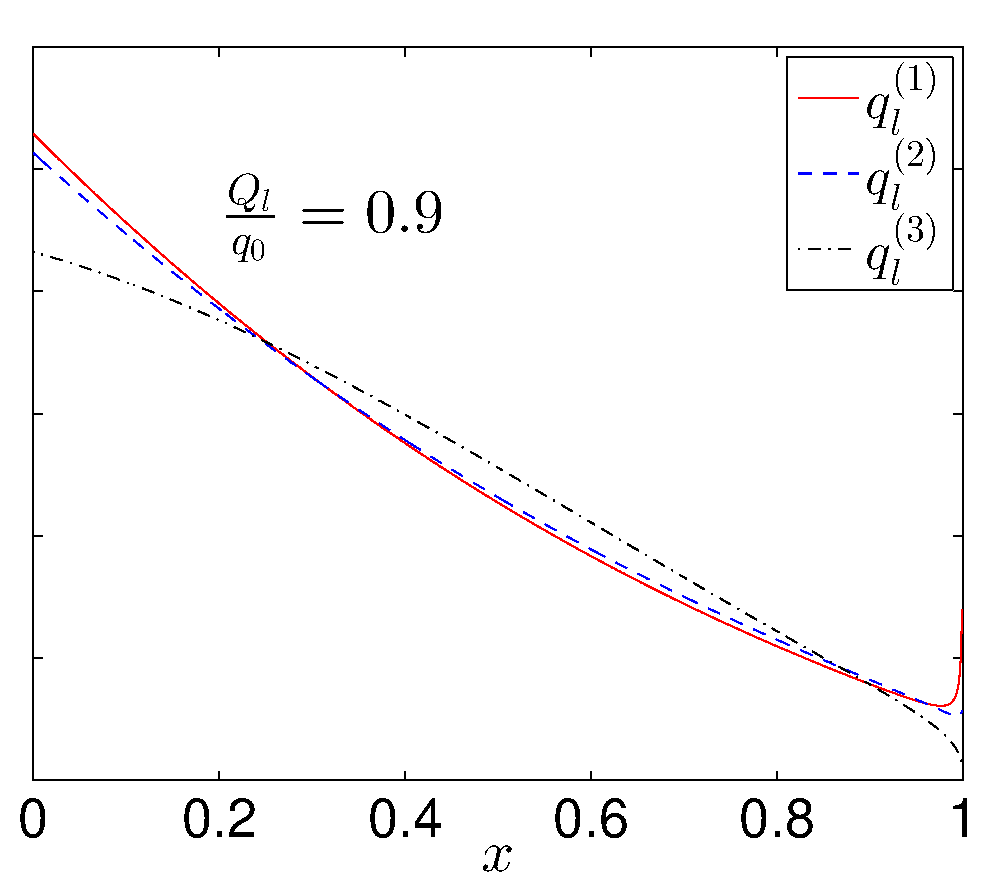
\includegraphics[width=\textwidth]{3_PKN_numerical/benchmark/leak11.eps}

 \end{subfigure}
 \begin{subfigure}{0.32\textwidth}
                \centering
                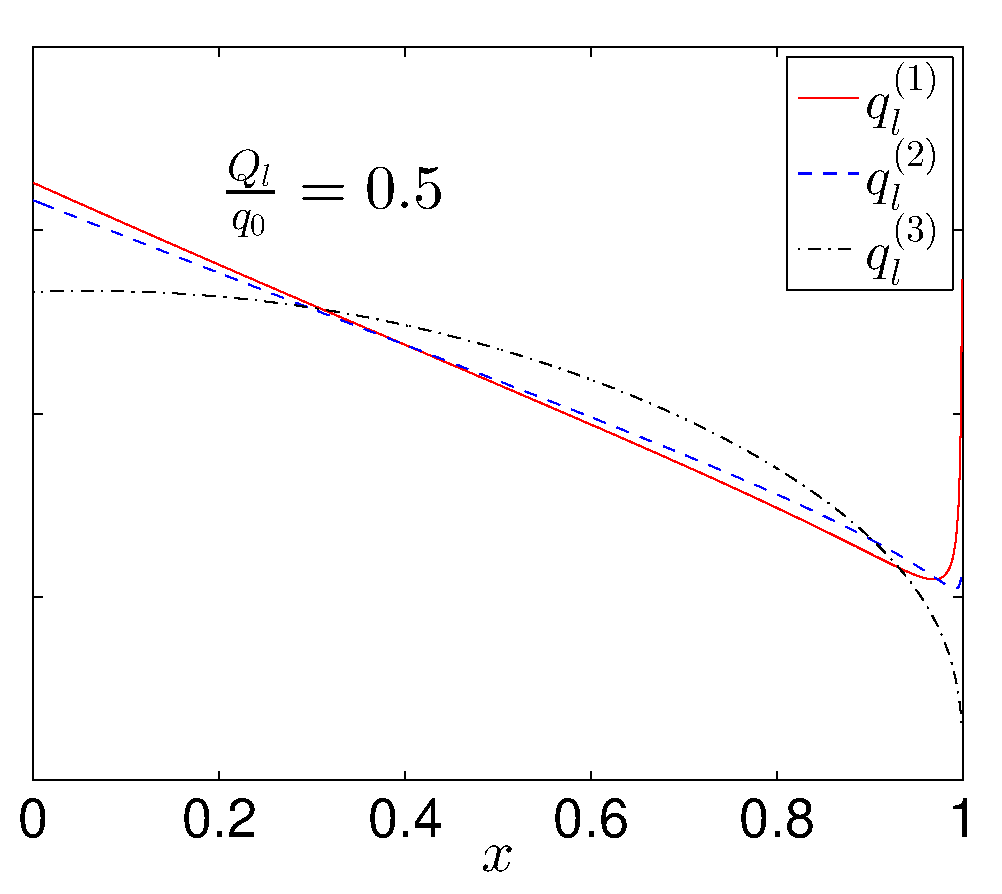
\includegraphics[width=\textwidth]{3_PKN_numerical/benchmark/leak12.eps}

\end{subfigure}
 \begin{subfigure}{0.32\textwidth}
                \centering
                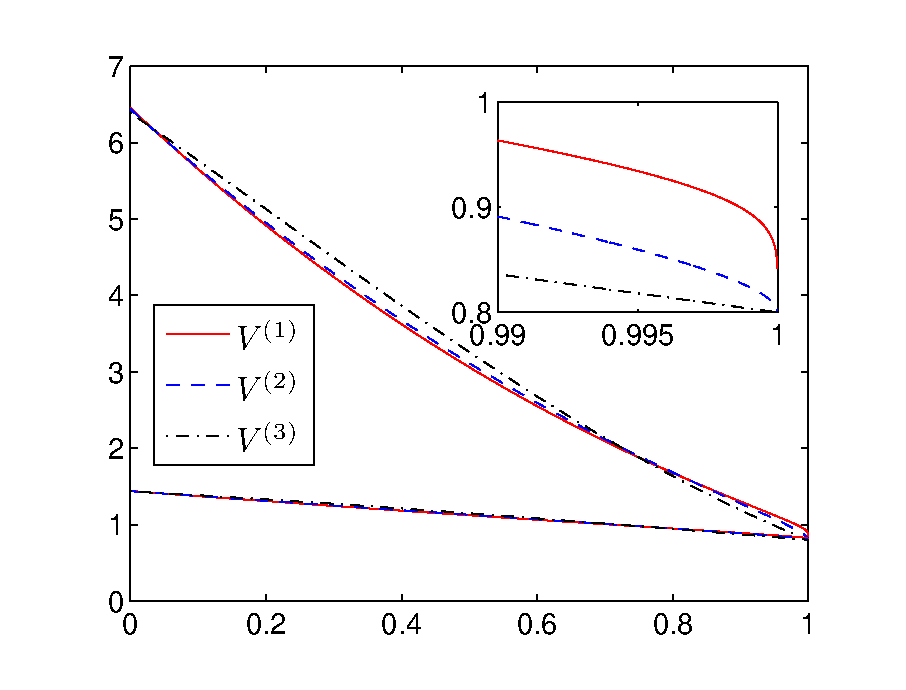
\includegraphics[width=\textwidth]{3_PKN_numerical/benchmark/V_graphs.eps}
                \begin{picture}(0,0)(0,0)
                \put(-40,35){\line(2,1){11}}
                \put(-50,29){${}_{Q_l/q_0=0.5}$}
                \put(-45,112){${}_{Q_l/q_0=0.9}$}
                \put(-40,100){\line(2,1){10}}
     \end{picture}
\begin{picture}(0,0)(405,-117)
   \put(50,-15){$Q_l/q_0=0.9$}     \put(215,-15){$Q_l/q_0=0.5$}
        \put(3,10){a)} \put(168,10){b)} \put(333,10){c)}
        \put(5,-35){$q_l$}      \put(170,-35){$q_l$} \put(332,-35){$V$}
        \put(80,-110){$x$}    \put(245,-110){$x$} \put(411,-110){$x$}
                \end{picture}
                \vspace{-2mm}
\end{subfigure}
\caption{Distributions of the leak-off functions $q_l(t,x)$ and the respective particle velocity $V(t,x)$ over $\tilde x \in(0,1)$ at initial time $t=0$.}
\label{fig:leak_offs}
\end{figure*}





Note also, that by manipulating with the value of $\gamma$ one can
simulate some very specific regimes of crack propagation. For
example $\gamma=1/5$ corresponds to the constant injection flux
rate, while $\gamma=1/3$ gives a constant crack propagation speed.
For our computations we always
set the value of $\gamma=1/5$.

Choosing appropriate values $b_1$ and $b_2$ one can change the relation between the amount of fluid loss to formation and the injection rate. This ratio can be defined by the  measure, $Q_l/q_0$, where $Q_l$ is the total volume of leak-off $\int_0^1 q_l dx$.
It is important to note that this measure decreases in time, from its maximum value to zero, for all chosen benchmarks. Thus, taking the maximal value high enough and tracing the solution accuracy in time, one can analyse performance of the algorithm for any possible value of the parameter. We consider two variants of $Q_l/q_0$,
one where fluid injection doubles the size of total fluid loss, and a second where the total fluid loss is close to injection rate.
The values of the corresponding parameters $b_1$, $b_2$ are presented in Table~\ref{tab_last}.
\begin{table}[h]
\centering
\begin{tabular}{c|c|c|c|c|c|c|}
\cline{2-7}
& \multicolumn{3}{c|}{$Q_l/q_0=0.9$ } & \multicolumn{3}{c|}{$Q_l/q_0=0.5$} \\ [.05in]\cline{2-7}
& $q_l^{(1)}$ & $q_l^{(2)}$ & $q_l^{(3)}$ & $q_l^{(1)}$ & $q_l^{(2)}$ & $q_l^{(3)}$ \\ [.05in]\cline{1-7}
\multicolumn{1}{|c|}{$b_1$} & $0.1$ & $0.19$ & $0.74$ &$0.02$& $0.03$& $0.15$ \\[.02in]\cline{1-7}
\multicolumn{1}{|c|}{$b_2$} &$0.5$ & $0.41$& $-0.13$ &$0.1$& $0.08$& $-0.02$ \\ \cline{1-7}
\multicolumn{1}{|c|}{ $\gamma_v$} &$1.69$ & $1.70$& $1.65$ &$0.55$& $0.56$& $0.55$ \\ \cline{1-7}
\end{tabular}
\caption{The values of parameters $b_1$ and $b_2$ for different benchmark solutions modelling desired leak-off to fluid injection ratios.}
\label{tab_last}
\end{table}



Additionally one can compute a parameter $\gamma_v$ defined in \cite{MWL} as a measure of the uniformity of fluid velocity distribution:
%\begin{equation}\label{gamma_v}
%\begin{split}
\begin{equation}
\label{gamma_v}
\gamma_v=\left[\max(V(t,x))-\min(V(t,x))\right]\left[\int_0^1V(t,\xi)d\xi\right]^{-1}.
\end{equation}
%\end{split}
%\end{equation}
Interestingly, this measure is directly correlated with the leak-off ratio $Q_l/q_0$.

In Fig.~\ref{fig:leak_offs} the distributions  of the leak-off functions and the corresponding particle velocities for the respective benchmarks are presented.
It shows that the velocity near the crack tip depends strongly on the benchmark variant. To highlight this fact, a zoom picture is placed in the Fig.~\ref{fig:leak_offs} b).

Note that the benchmark $q_l^{(1)}$ is worse, in a sense, than the original Carter's model as it contains additional singular terms of the leak-off function.
These terms are absent in the normalised Carter's law as it follows from Appendix B.

\subsubsection{General Benchmark}
We should construct our own benchmark solution that satisfies the proposed problem. The function $w(\tilde x,t)$ should be written as: 
  
\begin{equation}\label{w_bench}
w(\tilde x,t)=U_0(a+t)^\gamma w_0(x)
\end{equation}

Where $U_0$,$a$,$\gamma$ are arbitrary parameters, and function $w_0(\tilde x)$ is given an $n$ term sum:
\begin{equation}\label{w_bench}
w_0(\tilde x)=\sum_{j=0}^n A_j(1-\tilde x)^{\alpha_j}
\end{equation}
We have previously found that we need to begin at $\alpha_{0}=\frac{1}{3}$ and flowing powers of $\alpha_j$ increase by $\frac{1}{6}$ when writing down asymptotic expansion [ref??]. Now from the speed equation \eqref{speed} we write:

\begin{equation}\label{v_bench}
V(\tilde x,t)=-\frac{kU_0^3}{ML(t)}(a+t)^{3\gamma}w_0(x)^2\frac{\partial w_0}{\partial \tilde x}
\end{equation}
And so the speed at crack tip $\tilde x=1$ is given by
\begin{equation}\label{v_1_bench}
V(1,t)=\frac{k U_0^3}{3ML(t)}(a+t)^{3\gamma}
\end{equation}
Furthermore from relation \eqref{???}  and \eqref{???}:

\begin{equation}\label{L_bench}
L(t)=\sqrt{\frac{2kU_0^3}{3M(3\gamma+1)}}(a+t)^{\frac{3\gamma+1}{2}}
\end{equation}

\begin{equation}\label{q_0_bench}
q_0(t)=-\sqrt{\frac{3(3\gamma+1)kU_0^5}{2M}}(a+t)^{\frac{5\gamma-1}{2}}w_0^3(0)\frac{\partial w_0}{\partial \tilde x}|_{\tilde x=0}
\end{equation}

Substitution of \eqref{w_bench} into our problem equation \eqref{???} allows us to write $q_l(\tilde x,t)$ in terms of $w_0$ and its derivatives:

\begin{equation}\label{q_l_bench}
q_l(\tilde x,t)=U_0(a+t)^{\gamma-1}\left(\frac{3}{2}(3\gamma+1)\left(\frac{1}{3}x\frac{\partial w_0}{\partial \tilde x}+3w_0^2\frac{\partial w_0}{\partial \tilde x}^2+w_0^3\frac{\partial^2 w_0}{\partial \tilde x^2}\right)-\gamma w_0\right)
\end{equation}

\subsubsection{2 terms benchmark}
We can write a simple form of the above benchmark by using only two terms of $w_0$ and choosing $A_0=1$, then we have:
\begin{equation}\label{w_2_bench}
w_0(\tilde x)=(1-\tilde x)^{\frac{1}{3}}+A_1(1-\tilde x)^{\frac{1}{2}}
\end{equation}
Therefore we can write down $q_l(\tilde x,t)$ simply as:
\begin{align}\label{q_l_2_bench}
q_l(\tilde x,t)=U_0(a+t)^{\gamma-1}&\Bigg[(3\gamma+1)\left(\frac{7}{8}A_1(1-\tilde x)^{-\frac{1}{2}}+\frac{5}{2}A_1^2(1-\tilde x)^{-\frac{1}{3}}+\frac{55}{24}A_1^3(1-\tilde x)^{-\frac{1}{6}}+\frac{3}{4}A_1^4(1-\tilde x)^{0}\right)
 \nonumber \\
&+\frac{1}{6}(1-3\gamma)(1-\tilde x)^{\frac{1}{3}}+\frac{1}{4}(1-\gamma)A_1(1-\tilde x)^{\frac{1}{2}}\Bigg]
\end{align}

Having written so we can find that the lowest term $(1-x)^{-1/2}$ is multiplied by $\frac{7}{8}U_0(3\gamma-1)(a+t)^{\gamma -1}$. If we consider our results form asymptotic \eqref{???} we can match these coefficient with $DC(t)$ that comes with the same power. Therefore substituting \eqref{L_bench} into \eqref{C_t}:

\begin{equation}\label{C_t_bench}
C(t)=\sqrt{\frac{3\gamma+1}{2}}(a+t)^{-\frac{1}{2}}
\end{equation}

This allows us to find $D$ which is:
\begin{equation}\label{D_bench}
D=A_1\frac{7\sqrt{2}}{8}U_0(3\gamma+1)^{\frac{1}{2}}(a+t)^{\gamma-\frac{1}{2}}
\end{equation}

The value of $D$, which has a physical meaning of material permeability can be a constant parameter with choice $\gamma =\frac{1}{2}$. (???? ma to sens ????) Different values of $\gamma$ 
would give less realistic model when the material changes its properties during hydrofracturing. These however would still give a "good" mathematical model.

